\chapter{Ergebnisse}

\section{Prinzipielle Auswirkungen von ADC Clock Phasenrauschen auf die MRT Bildqualität}
In diesem Abschnitt wird zunächst qualitativ dargestellt, wie sich das Phasenrauschen des ADC Clock-Signals auf die Qualität eines rekonstruierten MRT Schichtbildes auswirkt.

Als Referenz dient die Simulation in \autoref{fig:inputPhantom}. Die Aufnahme des Referenzbildes erfolgt mit einer Gradientenecho-Sequenz und einer Auflösung von 200x160 Pixeln. Die Schichtdicke beträgt \SI{6}{\mm}. Vor dem Rekonstruktionsschritt wird weder Amplituden- noch Phasenrauschen zum MR-Signal hinzugefügt.

\begin{figure}[H]
	\centering
	\adjincludegraphics[width=0.45\textwidth,trim={{0.135\width} {0.1\height} {0.25\width} {0.15\height}},clip]{img/results/input.png}
	\caption[Referenz für die Simulation]{Referenzbild für die weiteren Betrachtungen, Gradientenecho-Sequenz, Auflösung 200x160px}
	\label{fig:inputPhantom}
\end{figure}

\subsection{Gradientenecho-Sequenz}
Zunächst wird das MR-Signal, dass durch die Simulation einer Gradientenecho-Pulssequenz gewonnen wird, mit einem weißen, Gauß-verteilten Phasenrauschen versehen:
\begin{equation}
	\label{eq:greWhite}
	\Delta \Phi(t)=\Delta \Phi[n]=X_{\xi}[n], \quad X \sim N(0,1)
\end{equation}
Das rekonstruierte Bild und der Verlauf von $\Delta \Phi(t)$ sind in \autoref{fig:GREwhite} dargestellt.

\begin{figure}[H]
	\centering
	\subcaptionbox{Rekonstruiertes Schnittbild}{\adjincludegraphics[width=0.45\textwidth,trim={{0.135\width} {0.1\height} {0.25\width} {0.15\height}},clip]{img/results/white.png}}
	\hfill
	\subcaptionbox{Zeitverlauf von $\Delta \Phi(t)$}{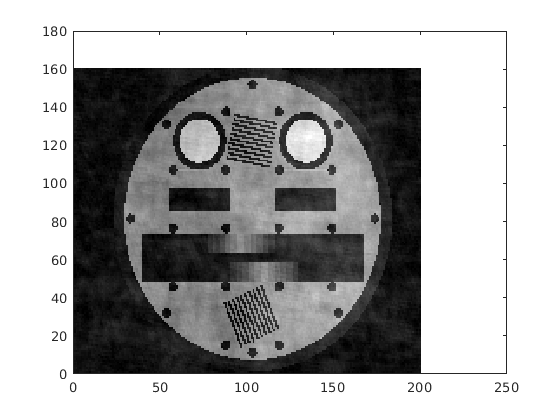
\includegraphics[width=0.45\textwidth,height=0.4\textwidth]{img/results/white.tikz}}
	
	\caption{Weißes Phasenrauschen bei einer GRE-Sequenz}
	\label{fig:GREwhite}	
\end{figure}

Wird das weiße Rauschen aus \autoref{eq:greWhite} integriert, entsteht $1/f$-Rauschen:
\begin{equation}
	\label{eq:brown}
	\Delta \Phi(t)=\Delta \Phi[n]= \sum_{i=0}^{n} X_{\xi}[i], \quad X \sim N(0,1)
\end{equation} 

\autoref{fig:greoneOverf} zeigt das dazugehörige rekonstruierte Bild zusammen mit dem Verlauf von $\Delta \Phi(t)$.

\begin{figure}[H]
	\centering
	\subcaptionbox{Rekonstruiertes Schnittbild}{\adjincludegraphics[width=0.45\textwidth,trim={{0.135\width} {0.1\height} {0.25\width} {0.15\height}},clip]{img/results/oneOverF_weak.png}}
	\hfill
	\subcaptionbox{Zeitverlauf von $\Delta \Phi(t)$}{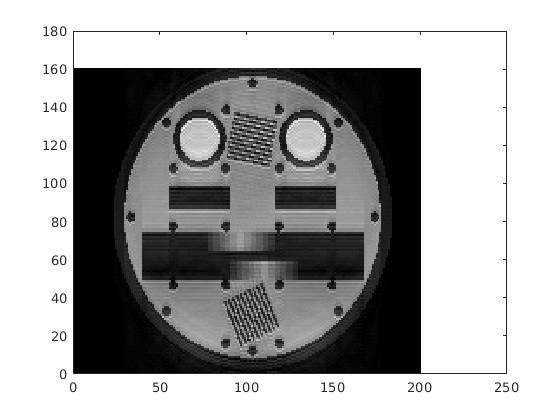
\includegraphics[width=0.45\textwidth,height=0.4\textwidth]{img/results/oneOverF_weak.tikz}}
	\label{fig:greoneOverf}
	\caption{$1/f$-Phasenrauschen bei einer GRE-Sequenz}	
\end{figure}

\subsection{Echo-Planar-Sequenz}

Die Phasenrausch-Simulationen aus \autoref{eq:greWhite} und \autoref{eq:brown} werden mit einer EPI-Pulssequenz wiederholt. Die Ergebnisse zeigen \autoref{fig:epiWhite} und \autoref{fig:epiOneoverF}.

\begin{figure}[H]
	\centering
	\subcaptionbox{Rekonstruiertes Schnittbild}{\adjincludegraphics[width=0.45\textwidth,trim={{0.135\width} {0.1\height} {0.15\width} {0.15\height}},clip]{img/results/epiWhite.png}}
	\hfill
	\subcaptionbox{Zeitverlauf von $\Delta \Phi(t)$}{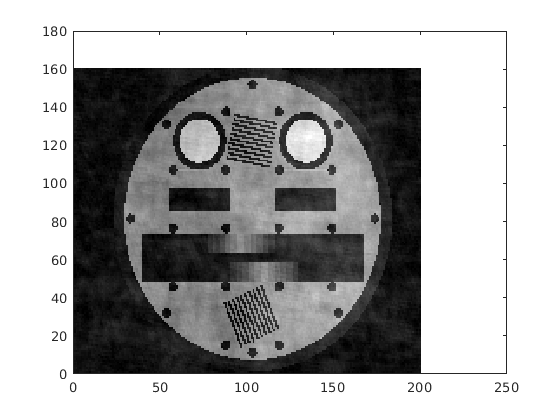
\includegraphics[width=0.45\textwidth,height=0.4\textwidth]{img/results/white.tikz}}
	
	\caption{$1/f$-Phasenrauschen bei einer EPI-Sequenz}
	\label{fig:epiWhite}	
\end{figure}

\begin{figure}[H]
	\centering
	\subcaptionbox{Rekonstruiertes Schnittbild}{\adjincludegraphics[width=0.45\textwidth,trim={{0.135\width} {0.1\height} {0.15\width} {0.15\height}},clip]{img/results/epiOneOverF.png}}
	\hfill
	\subcaptionbox{Zeitverlauf von $\Delta \Phi(t)$}{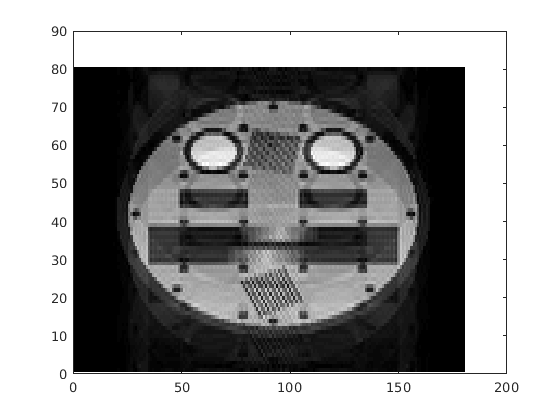
\includegraphics[width=0.45\textwidth,height=0.4\textwidth]{img/results/epiOneOverF.tikz}}
	
	\caption{$1/f$-Phasenrauschen bei einer EPI-Sequenz}
	\label{fig:epiOneoverF}	
\end{figure}

\autoref{fig:epiSine} zeigt eine Sinus-förmige Modulation der Phase des MR-Signals. Die Modulation ist gegeben durch:
\begin{equation}
	\Delta \Phi(t)=\Delta \Phi[n]= \beta sin(2 \pi \nu_m t), \quad t=(0,\frac{1}{f_{receiver}},\frac{2}{f_{receiver}},...,\frac{N-1}{f_{receiver}})
\end{equation}
Im Beispiel in \autoref{fig:epiSine} wird als Modulationsfrequenz $\nu_m=\SI{10}{\kilo\hertz}$ und als Modulationsfaktor $\beta=0.1 \pi$ verwendet.

\begin{figure}[H]
	\centering
	\subcaptionbox{Rekonstruiertes Schnittbild}{\adjincludegraphics[width=0.45\textwidth,trim={{0.135\width} {0.1\height} {0.15\width} {0.15\height}},clip]{img/results/sine.png}}
	\hfill
	\subcaptionbox{Zeitverlauf von $\Delta \Phi(t)$}{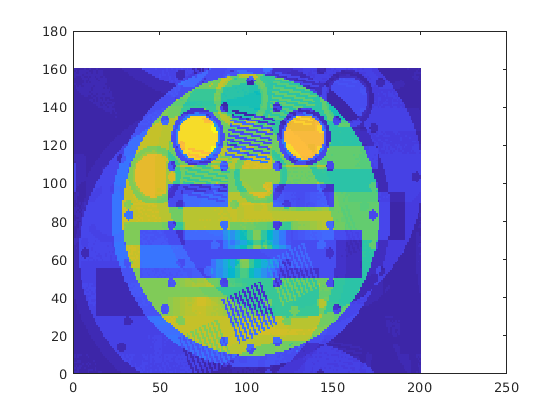
\includegraphics[width=0.45\textwidth,height=0.4\textwidth]{img/results/sine.tikz}}
	
	\caption{Sinus-förmige Modulation der Phase bei einer EPI-Sequenz}
	\label{fig:epiSine}	
\end{figure}














